\scanpage{97}
\mspage{96}
$\mathcal E$-structure
\[
(21)\qquad \mathcal E\longrightarrow\operatorname{Aut}\operatorname{id}_{\Pi_1(P_0)}
\]
\unsure{Alors} si $x_0,y_0\in P_0$, $\mathcal E$ opère librement sur
$\operatorname{Hom}_{\Pi_1(P_0)}(x_0,y_0)$ à droite (via son op. sur $x$) et à
gauche (via son opération sur $y$), les deux
structures \deleted{étant} se correspondent via \uuline{la}
\deleted{\unsure{même}} formule
\[
\ell\mathbin{.}\gamma_{x_0}=\deleted{\unsure{\gamma}}\,{}^\ell\gamma_{y_0}\mathbin{.}\ell
\qquad(\ell\in\operatorname{Hom}(x_0,y_0),\ \gamma\in\pi)
\]
\[
\text{où}\quad \deleted{\unsure{\mathcal E}}\,{}^\ell\gamma_{y_0}=\ell\mathbin{.}\gamma\mathbin{.}\ell^{-1}
\]
\figure{\begin{tikzpicture}[x=.4cm,y=.4cm]\draw[dashed] (0,0)--(2,0);\end{tikzpicture}}
\deleted{Si $x,y\in P$, alors}
L'image inverse du groupoïde $\Pi_1(P_0)$
par l'application \deleted{\unsure{Alors}} \inserted{$q:P\mathbin{\text{---}}P_0$} sur l'ens des objets
n'est autre que $\Pi_1(P)\mathbin{\wedge}_{\pi}\mathcal E$. Donc
l'image inverse de $\Pi_1(P_0)$ par la composée
\[
E\mathbin{\text{---}}P\mathbin{\xrightarrow{q}}P_0
\]
n'est autre que
$C'\mathbin{\wedge}_{\pi}\mathcal E$,
\deleted{et alors \unsure{le|la} \inserted{\unsure{structure de}} $\mathcal E$-groupoïde \unsure{obtenu}}
\unsure{qui peut s'obtenir ainsi}
\deleted{quotient}
\inserted{directement} à partir du groupoïde $C_0$ image
\inserted{inverse de} $\Pi_1(P_0)$ par l'application
\deleted{\unsure{Ob}} $E_0\longrightarrow P_0$. Je
\margin{\figure{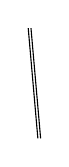
\begin{tikzpicture}[x=.35cm,y=.35cm]\draw (0,0)--(-.35,4);\draw (.1,0)--(-.25,4);\end{tikzpicture}}}
dis que \unsure{cette|ce} $C_0$ peut se construire de
façon purement algébrique en termes de
$C'$ muni des structures de $\pi$-groupoïde à
groupe d'opérateurs $\mu$, \inserted{et de la structure d'ext. (13)}, \unsure{comme}
